\documentclass[a4paper, 12pt]{report}
\usepackage[a4paper,hmargin={3cm,2.5cm},vmargin={2.5cm,2.5cm}]{geometry}
\usepackage{amsfonts} % if you want blackboard bold symbols e.g. for real numbers
\usepackage{graphicx} % if you want to include jpeg or pdf pictures
\usepackage{multicol}
\usepackage[export]{adjustbox}
\usepackage{lipsum}
\usepackage{subfig}
\usepackage{float}
\usepackage{blindtext}
\usepackage{fancyhdr}
\usepackage{multirow}
\pagestyle{fancy}
\lhead{}
\rhead{Wine Prediction Quality}
\lfoot{Dept. of Information Technology}
\usepackage{tikz}
\usepackage{tabularx}
\usetikzlibrary{calc}
\usepackage{eso-pic}
\usepackage{lipsum}
\usepackage{longtable}
\usepackage{listings}
\renewcommand{\bibname}{References}
\begin{document}
%========================================================= %
%================begin of title page====================== %
% The frontmatter environment for everything that comes with roman numbering\
%============================================= %
\newenvironment{frontmatter}{}{}
\begin{frontmatter}
%%%%%%%%%%%%%%%%%%%%%%%%%%%%%%%%%%%%%%%%%%%%%%%%%%%%%%%%%%%%%%%%%%%
\begin{titlepage}
%\AddToShipoutPictureBG
\begin{center}

%---------------------------------Figure------------------------------

\begin{center}
\begin{figure}[h]  %h means here other options t , b, p, etc.
\centering

\includegraphics[width=0.2\linewidth]{./veslogo}
\end{figure}
\end{center}

%----------------------------
\textup{\large PROJECT REPORT\\[0.4cm]ON}\\[0.4cm]
\begin{LARGE}
{\textbf {Wine Quality Prediction }}\end{LARGE}\\[1cm]
\textup{\large  SUBMITTED IN PARTIAL FULFILLMENT OF THE REQUIREMENT FOR SEMESTER V OF }\\[0.6cm]
\begin{large}\textbf {T.E.(Information Technology)}
\end{large}\\[0.5cm]
\textit{SUBMITTED BY}\\[0.2cm]
\begin{large}
\\ \textbf{Miss. Aditi Miniyar (IT5B114)}\\[0.7cm]
\textbf{Mr. Jayesh Rajput (IT5B130)}\\[0.7cm]
\textbf{Miss. Ghanishtha Talele (IT5B132)}\\[0.7cm]
\textbf{Mr. Vinit Variyani (IT5B135)}\\[0.7cm]
\end{large}
\textit{UNDER THE GUIDANCE OF}\\[0.1cm]
\begin{large}\textbf{PROF.Charusheela Nehete }\\[0.2cm]\end{large}

\vfill
\textbf{DEPARTMENT OF INFORMATION TECHNOLOGY\\
V.E.S. INSTITUTE OF TECHNOLOGY\\
2022-23
\end{center}

}
\end{titlepage}
%================begin of certificate page======================

\begin{titlepage}
\begin{tikzpicture}[overlay,remember picture]
\draw[line width=4pt]
    ($ (current page.north west) + (1cm,-1cm) $)
    rectangle
    ($ (current page.south east) + (-1cm,1cm) $);
\draw[line width=1.5pt]
    ($ (current page.north west) + (1.2cm,-1.2cm) $)
    rectangle
    ($ (current page.south east) + (-1.2cm,1.2cm) $);
\end{tikzpicture}
\begin{center}

\begin{LARGE}
\textbf{\textit {Certificate}}\end{LARGE}\\[0.5cm]
This is to certify that project entitled\\[0.5cm]\large\textbf{ "Wine Quality Prediction"}\\[0.5cm]

\textbf{Group Members Names}\\
Miss. Aditi Miniyar ( Roll No. 44 ) \\
Mr. Jayesh Rajput ( Roll No. 60 ) \\
Miss. Ghanishtha Talele  ( Roll No. 63 ) \\
Mr. Vinit Variyani ( Roll No. 67 ) \\
\end{center} 
In partial fulfillment of degree of TE. (Sem V) in Information Technology for  Project is approved.
\vspace{2cm}
\begin{multicols}{2}
\begin{center}
\textbf{Prof.Charusheela Nehete \\Project Mentor}\hspace{8cm}\\
\end{center}
\begin{center}
\textbf{External Examiner}\hspace{8cm}\\
\end{center}
\end{multicols}
\vspace{0.6cm}
\begin{multicols}{2}
\begin{center}
\textbf{Dr.(Mrs.)Shalu Chopra\\H.O.D}\hspace{8cm}\\
\end{center}
\begin{center}
\textbf{Dr.(Mrs.)J.M.Nair\\ Principal}\\
\end{center}
\end{multicols}
\vfill
\vspace{0.5cm}
\text{Date: / /2022}\\
\text{Place: VESIT, Chembur}\\
\begin{flushright}
College Seal
\end{flushright}

\end{titlepage}


%================end of title page======================
%----------------------ACKNOWLEDGEMENT---------------------------
\pagenumbering{gobble}

\pagebreak


\newpage
\begin{center}
{\Large{\bf{\textit{Declaration}}\\[2cm]}}
\end{center}
I declare that this written submission represents my ideas in my own words and where others' ideas or words have been included, I have adequately cited and referenced the original sources. I also declare that I have adhered to all principles of academic honesty and integrity and have not misrepresented or fabricated or falsified any idea/data/fact/source in my submission. I understand that any violation of the above will be cause for disciplinary action by the Institute and can also evoke penal action from the sources which have thus not been properly cited or from whom proper permission has not been taken when needed. 


\vspace{0.8in}
\begin{flushright}
- - - - - - - - - - - \\
\textbf{(Signature)}\\
\vspace{0.2in}
Aditi Miniyar (Roll No.44)\\
\end{flushright}

\vspace{0.6in}
\begin{flushright}
- - - - - - - - - - - \\
\textbf{(Signature)}\\
\vspace{0.2in}
Jayesh Rajput (Roll No.60)\\
\end{flushright}

\vspace{0.6in}
\begin{flushright}
- - - - - - - - - - - \\
\textbf{(Signature)}\\
\vspace{0.2in}
Ghanishtha Talele (Roll No.63)\\
\end{flushright}

\vspace{0.6in}
\begin{flushright}
- - - - - - - - - - - \\
\textbf{(Signature)}\\
\vspace{0.2in}
Vinit Variyani (Roll No.67)\\
\end{flushright}

\pagenumbering{roman}
\setcounter{page}{1}

\newpage
\begin{center}
{\Large{\bf{\textbf{ACKNOWLEDGEMENT}}\\[2cm]}}
\end{center}
The project report on " Wine Quality Prediction " is the outcome of the guidance, moral support and devotion bestowed on our group throughout our work. For this we acknowledge and express our profound sense of gratitude to everybody who has been the source of inspiration throughout project preparation. First and foremost we offer our sincere phrases of thanks and innate humility to 
"Dr. Shalu Chopra HOD-IT", "Manoj Sabnis Deputy HOD", "Charusheela Nehete
Assistant Professor" for providing the valuable inputs and the consistent guidance and support provided by them.We can say in words that we must at outset tender our intimacy for receipt of affectionate care to Vivekanand Education Society's Institute of Technology  for providing such a stimulating atmosphere and conducive work environment.

\pagenumbering{roman}
\setcounter{page}{2}

%%%%%%%%%%%%%%% Abstract %%%%%%%%%%

\newpage
\begin{center}
{\Large{\bf{\textbf{Abstract}}\\[2cm]}}
\end{center}
\par Wine quality is essential for both consumers and the wine industry. The traditional (expert) method of determining wine quality takes time. Machine learning models are now essential tools for replacing human tasks. In this instance, there are several features that can be used to predict wine quality, but not all of them will be useful. As a consequence, our thesis work focuses on what wine characteristics are important to achieve a promising result. We used three methods for the classification model and feature evaluation, namely support vector machine (SVM) and naive Bayes(NB). We used two wine quality databases in this study: red wine and white wine. To compare the machine learning algorithm, we used the Pearson coefficient correlation and performance measurement matrices such as accuracy, recall, precision, and f1 score to analyze feature importance. To enhance model accuracy, a grid search algorithm was used. Finally, we discovered that the Random Forest algorithm outperformed the Decision Tree, AdaBoost  algorithm, and Gradient boosting Algorithm for both red and white wine datasets. 

\vspace{0.3cm}

\textbf{Keywords-}\it{\textbf{literature, theoretical, methodological, include, Publication}
\end{frontmatter}


\newpage
\tableofcontents
\listoffigures
\listoftables
\lfoot{}
% %%%%%%%%%%%%%%% Abstract %%%%%%%%%%
% %\newpage
% \begin{abstract}
% \par Abstract Here\\
% \vspace{0.3cm}

% \textbf{Keywords-}\it{\textbf{smoke detector alarm , Fire detector , Arduino , MQ2 Smoke sensor.}\\
% \end{abstract}
% %================================================ %
% % The frontmatter environment for everything that comes with roman numbering %
% \end{frontmatter}
% %%%%%%%%%%%%%%%%%%%%%%%%%%%%%%%%%%%%%%%

\newpage
\pagenumbering{arabic}
%%%%%%%%% MAIN TEXT STARTS HERE %%%%%%%%%%
\chapter{Introduction}

\section{Introduction }
\par In recent years, there has been a notable increase in wine consumption, driven by both the leisurely enjoyment of wine and the health benefits it offers, particularly in terms of heart health. As with any industry, winemakers are constantly seeking to improve their methods and techniques to increase output and efficiency, while also meeting the growing demands of consumers. However, these improvements come at a cost, with rising expenses associated with implementing new procedures. Despite this, wine remains a popular beverage with a variety of functions.
\par The chemicals used in winemaking are largely the same across different varieties, although the specific chemicals used may vary. To determine the quality of wine, it is important to evaluate various factors, including sensory data and physicochemical tests. However, each individual may have a unique perspective on the taste and quality of wine, making it challenging to assess wine quality based solely on human opinions. \par Every person has their own taste, so identifying a trait based on a person's taste is difficult. With the advancement of technology, manufacturers began to rely on different devices for testing during the development phases. As a result, they will have a better understanding of wine quality, which will save them both money and effort. Furthermore, this aided in the collection of a large amount of data with various parameters such as the quantity of different chemicals and temperature used during production, as well as the quality of the wine created. These data are accessible in a number of databases. With the rise and success of machine learning techniques over the last decade, there have been numerous attempts to determine wine quality using available data.



\section{Aim and Objectives  }
\par The objectives of this project are as follows:
\newline
1)To experiment with different classification methods to see which yields the highest accuracy
\newline
2)To determine which features are the most indicative of a good quality wine
\newline
\newline
Aim of this project:
% Create unordered list in LaTeX
\begin{itemize}
  \item To balance the dataset. 
  \item To analyze the impact of the features. 
  \item To optimize the classification models through hyperparameter tuning.  
  \item To model and evaluate the approaches.

 
\end{itemize}

\section{Motivation for the Work }
\par The quality of wine is a significant concern for both wine industry professionals and customers. Traditionally, wine quality has been assessed by experts, which is a time-consuming process. With the advent of machine learning models, it has become possible to automate this process to some extent, reducing the need for human involvement.
In our thesis work, we are focusing on predicting wine quality using machine learning models. One of the challenges in this task is identifying the characteristics of the wine that are most important in determining its quality. Not all features will be equally useful for making accurate predictions, so we need to identify the most relevant ones.
The quality of wine is influenced by a variety of factors, including the percentage of each entity contained in the wine. Our model's primary goal is to provide predictions based on input values, such as the percentage of different entities in the wine. In addition, our model will suggest changes that could be made to improve wine quality, such as increasing the percentage of a particular entity.
To achieve our goal, we are developing a user-friendly interface that will allow users to input data and receive predictions and recommendations in real-time. Our model will use machine learning algorithms to analyze the input data and generate predictions based on patterns it has learned from previous data. By providing users with this information, we hope to help them make better decisions about wine quality and improve the overall quality of the wine industry.
\section{Scope of Project}
\par The prediction of wine quality through machine learning algorithms has been a significant advancement in the wine industry. It has helped in reducing human errors and provided a more efficient way of quality control. However, the accuracy of the classifier can be enhanced by adjusting the algorithm or the data being used. To improve the accuracy of the algorithm, it is necessary to adjust the parameters and fine-tune the model. Alternatively, it may require the use of a different algorithm altogether. The algorithm used should be able to capture the subtle differences in the wine characteristics, and the choice of algorithm can vary depending on the type of wine being predicted. Comparing the performance of different algorithms is essential in identifying the most effective one for the data set. Furthermore, improving the data set is crucial in enhancing the accuracy of the classifier. The data set should be comprehensive and should include a wider range of characteristics. It may require collecting data from different regions or vineyards to capture the full range of variations in wine quality. The data set should also be refined to remove outliers and improve its quality. Additionally, other performance measurement and machine learning algorithms can be used to provide a clearer comparison of results. Metrics such as accuracy, precision, recall, and F1 score provide a more nuanced understanding of the algorithm's strengths and weaknesses and can help identify areas for improvement. User feedback can also be incorporated into the evaluation process, allowing for continuous improvement based on real-world usage. The research will be useful in assisting manufacturing industries in predicting the quality of various types of wine based on certain characteristics. This will help in ensuring the production of an excellent item that meets the industry's standard. Machine learning algorithms can provide a reliable and efficient tool for predicting quality, but it requires continuous improvement of both the algorithm and the data set being used.

\section{Contribution }
\par The project aims to contribute to the field of machine learning and data mining by exploring their potential for predicting and presenting the most accurate results possible. The advancement of computing from mainframes to PCs to cloud and now to artificial intelligence, with machine learning being a defining aspect, has allowed for self-learning computers and the processing of big data at a remarkable speed.
The project aims to utilize the concepts and ideas from machine learning to analyze large data sets and identify patterns and associations. Similarly, data mining will be used for data discovery and sorting to answer teething worries through data analysis. Both machine learning and data mining share similar methods and processes, but the type of data pre-processing and end goal may differ.
The project's contribution to the field of machine learning and data mining lies in its exploration of how these technologies can be harnessed to improve predictions and present more accurate results. By optimizing the algorithms and adjusting the data sets, the project aims to improve the accuracy of predictions and support decision-making processes for various industries. Ultimately, the project aims to provide a foundation for future research in machine learning and data mining, leading to advancements and innovations in the field.


\section{Organization of the report }

Chapter 1 : It consists of an Introduction, Aim and Objectives, Motivation for the Project, Scope of Project, Contribution and Organization of the Project.\newline
Chapter 2 : It is the literature survey part of the project. It consists of Intoduction and Problem Definition.\newline
Chapter 3 : It is the design and Implementation part of the project. It consits of proposed system, requirement gathering, hardware requirements,  software requirements, UML diagrams, algorithm, cost estimation and Feasibility Study\newline
Chapter 4 : Result and discussion consist of Code, software results, screenshots, Testing results, Test case Report and Additional details. .\newline
Chapter 5: Summary and Future scope are mentioned in this chapter.
 

\chapter{Literature Survey}
\section{Introduction }
\par The core of your project is to basically predict whether the wine is suitable for drinking or not. It does so by looking at the values of the parameter that have been entered in the fields and by comparing those values to the standard values of the parameter. The parameter values could also change as per the person, as each parameter adds a different flavour and taste to the wine. Thereby, a proper standard range of values are defined for each parameter. Based on this range, the wine would be either considered as good or bad. Prior to choosing this project, our research noticed a lot of working on this particular field but with low accuracy reports. This shows that no significant work has still been done into this field of industry. Till date, only subjective opinion of human tasters is taken into consideration. Kumar et al. (2020) have used prediction of red wine quality using its various attributes and for the prediction, they used random forest, support vector machine, and naive Bayes techniques (Kumar et al., 2020). They have calculated the performance measurement such as precision, recall, f1-score, accuracy, specificity, and misclassification error. Among these three techniques, they achieved the best result from the support vector machine as compare to the random forest and naive Bayes techniques. They achieved the accuracy of the support vector machine technique is 67.25%.
\\
\par The second finding in the wine quality prediction was done by Gupta, (2018). He  used important features from red wine and white wine quality using various machine learning algorithms such as linear regression, neural network, and support vector machine techniques. They used two ways to determine the wine quality. Firstly the dependency of the target variable on the independent variable and secondly predicting the value of the target variable and conclusion that all features are not necessary for the prediction instead of selecting only necessary features to predict the wine quality (Gupta, 2018). Gupta came down to a conclusion that not all features must be taken down into consideration in order to predict the quality of wine. Only some of the features are necessary for predicting the quality of the wine. Thereby, taking the value of only these factors is required and only their values of these factors must be compared with the standard value and the range of the values. The result will be determined on the basis of these parameters. This would also largely reduce the time required for performing the procedure. Definitely, a large increase in the accuracy of prediction model was seen. It was also noticed that the users/customers found now the prediction model easy to operate and work with. And so a increase in the use of that particular model for prediction was noticed.
\\
\par The third theory was given by Dahal et al., (2021) has predicted the wine quality based on the various parameters by applying various machine learning models such as rigid regression, support vector machine, gradient boosting regressor, and multi-layer artificial neural network. They compare the performance of the models to predict wine quality and from their analysis, they found gradient boosting regressor is the best model to other model performances with the MSE, R, and MAPE of 0.3741, 0.6057, and 0.0873 respectively(Dahal et al., 2021). Then, Er, and Atasoy, (2016) has proposed the method to classify the quality of the red wine and white wine using three machine learning algorithm such as k-nearest-neighborhood, random forest, and support vector machine. They used principal component analysis for the feature 7 selection and they have achieved the best result using the random forest algorithm (Er, 2016). Lee et al., (2015) has proposed a method decision tree-based to predict the wine quality and compare their approach using three machine learning algorithm such as support vector machine, multi-layer perceptron, and BayesNet. They found their proposed method is better compared to other stated methods (Lee et al., 2015).
\\
\par The findings of the our Literature Survey is: \\
\\
1. Practically there is no impact on quality due to the fixed acidity. \\
2. There are some negative connection with the quality which appears in volatile acidity. \\
3. There are many better wines available which appear to have higher grouping of Citric Acid. \\
4. These better wines appear to have higher liquor rates. \\
5. Even however it's a frail association, yet lower percent of Chloride appears to create better quality wines. \\
6. Better wines appear to have lower densities. In some cases,  higher liquor content is also seen. \\
7. Better wines appear to be more acidic. \\
8. Residual sugar nearly has no impact on the wine quality. \\

\pagebreak

\section{Problem Definition}
\par In industries, understanding the demands of wine safety testing can be a complex task for the laboratory with numerous analyses and residues to monitor. But, our application's prediction, provide ideal solutions for the analysis of wine, which will make this whole process efficient and cheaper with less human interaction. As of now Human tasters are used which is obviously a subjective technique.
A decision support system can incorporate an autonomous prediction system to improve performance quality and speed. If it is determined that a number of input variables are highly related to predicting wine quality, this knowledge can be applied to raise wine quality.
The first part is to study the importance of the parameters for the prediction of wine quality. 
The second part  is to show that does the wine on the basis of its entered parameters qualify on being a good wine or a bad wine. As the parameters to test the wine could have multiple values and would reside between a range of values, it is difficult to determine that whether the wine is completely good and drinkable. It could also be possible that due to one of the values that is minorily different it could directly show that the wine is a bad wine



\chapter{Design & Implementation}
\section{Proposed System }
\par Collect a big dataset of red wine samples with different characteristics such as acidity, pH, residual sugar, alcohol content, volatile acidity, sulphate, and so on. Include the subjective quality ranking of each wine, as determined by professional wine tasters or experts.
Preprocess the data by selecting features, tidying it, and normalising it. Statistical techniques or domain expertise can be used to find the most important features for predicting wine quality. Cleaning entails removing missing or incorrect data, whereas normalisation guarantees that all features have the same scale.Based on the nature of the issue and the data, choose suitable machine learning models, such as regression or classification models. Random Forest, Support Vector Machine, Logistic Regression, Decision Tree, and Nave Bayes are some common models for predicting wine quality. Divide the data into training and testing groups, and then train the chosen model(s) on the training data. Deploy the trained model(s) as a web application or API so that users can send wine samples and receive real-time quality predictions. Furthermore, the system can provide insights into the variables that influence wine quality.

\section{Requirement Gathering and Analysis }
\par The project was launched after a market analysis of already existing projects. Indian citizens can save their official papers in a concept called a "Digi-Locker" according to the kind of document. This enables the user to quickly access the papers stored on their portable device. Making the patients keep their reports in one location is the rationale behind the Medi-Lock initiative.
We used the Node.js framework and the MongoDB database to make the project's implementation simple and seamless. Node.js application installation is required for its implementation in our systems, and it completes the installation process by configuring the environment variables.
The OTP API was required for this project since it relies on an authentication service to make the website more safe and reliable. Here, we utilised an OTP API called D7, which functions as after entering a contact number, a user will then get an OTP on that number. The user will enter it in the specified field after receiving the OTP. If and only if the OTP entered is accurate, the user will be authorised.
The payment gateway uses the API that is employed. Users will be given a variety of options for document storage. It is determined by the size of the submitted documents. The API called RazorPay makes it easy to implement the payment gateway in our project.
We utilised the XYZ API to implement the storage of documents. An application programming interface (API) for cloud storage connects a locally installed application to a cloud-based storage system so that users may send and receive data as well as access and manipulate data held there. This API meets our demand for report storage.
 

\section{Hardware Requirement }
\begin{itemize}
  \item Laptop/Desktop
  \item Memory (RAM): 4GB of RAM required
  \item Processor: Intel Dual Core or AMD Ryzen or M series processor
\end{itemize}


\section{Software Requirement }
\begin{itemize}
  \item Frontend : Flask
  \item Code Editor : Visual Studio Code
  \item Environment : Google Colab, Jupyter Notebook
\end{itemize} 

\section{UML Diagrams}
\subsection{Block Diagram }
\begin{figure}[h]
\centering
\\
\includegraphics[width=0.8\linewidth]{./UML.png}
\\
\caption{Block Diagram}
\end{figure}
\pagebreak

\subsection{Class Diagram }
\begin{figure}[h]
\centering
\\
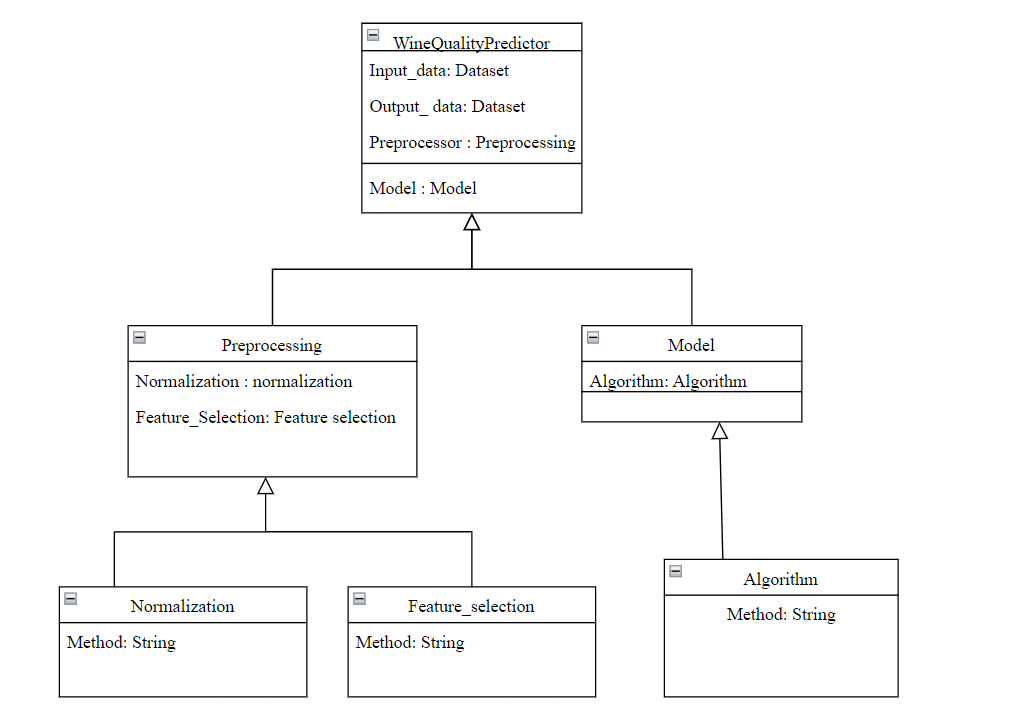
\includegraphics[width=0.9\linewidth]{./Wine Class diagram.png}
\caption{Class Diagram}
\end{figure}
\pagebreak
\subsection{Sequence Diagram }
\begin{figure}[h]
\centering
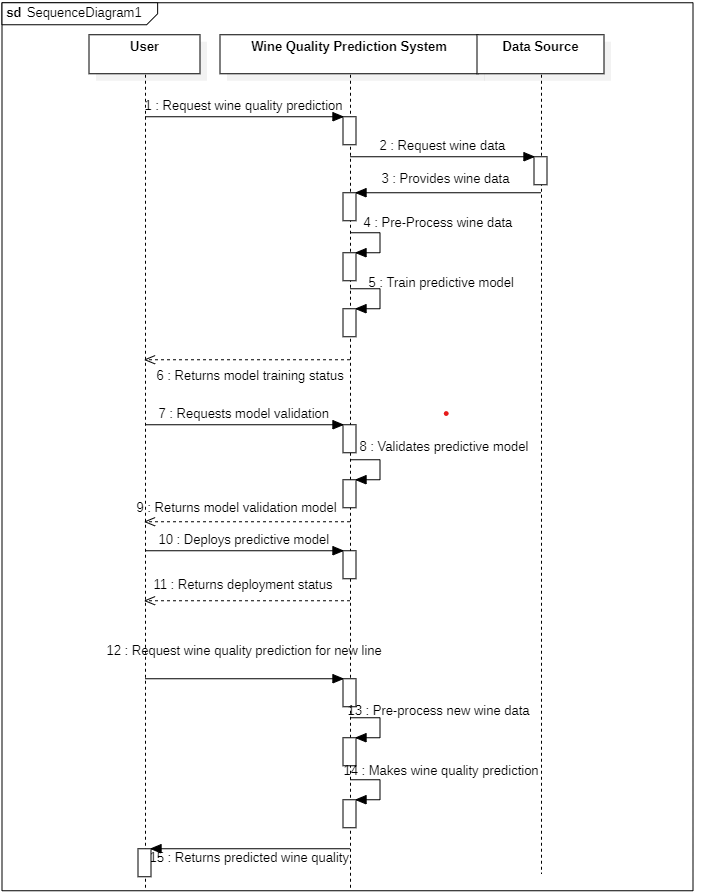
\includegraphics[width=0.9\linewidth]{./wine sequence daigram.png}
\caption{Sequence Diagram}
\end{figure}
\pagebreak

\subsection{Activity Diagram }
\begin{figure}[h]
\centering
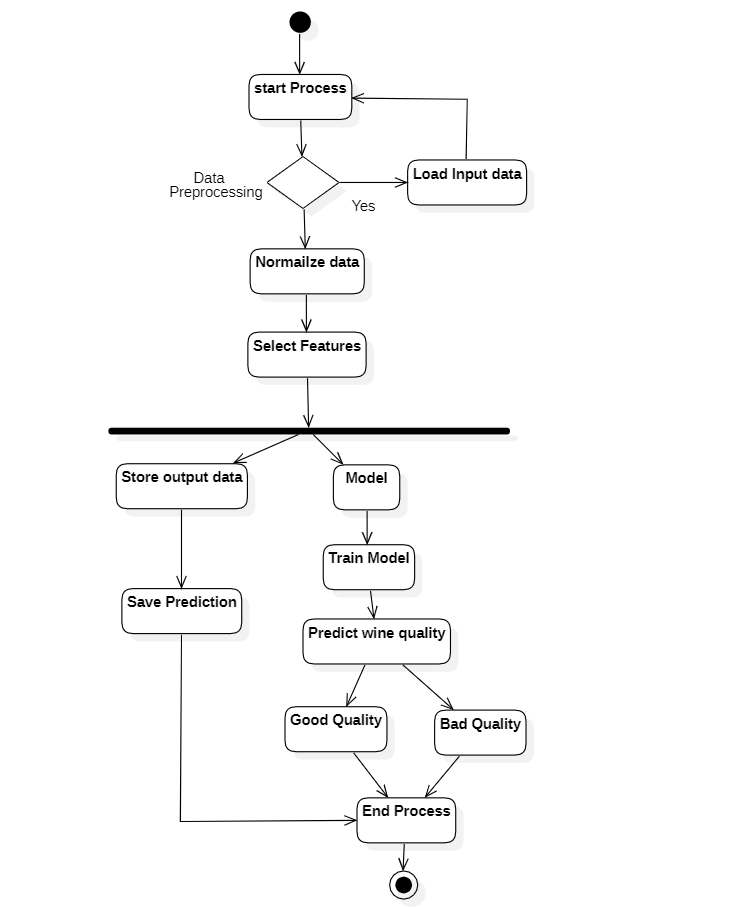
\includegraphics[width=1\linewidth]{./WINE ACTIVITY DIAGRAM.png}
\caption{Activity Diagram}
\end{figure}
\pagebreak

\subsection{Data Flow Diagram }
\begin{figure}[h]
\centering
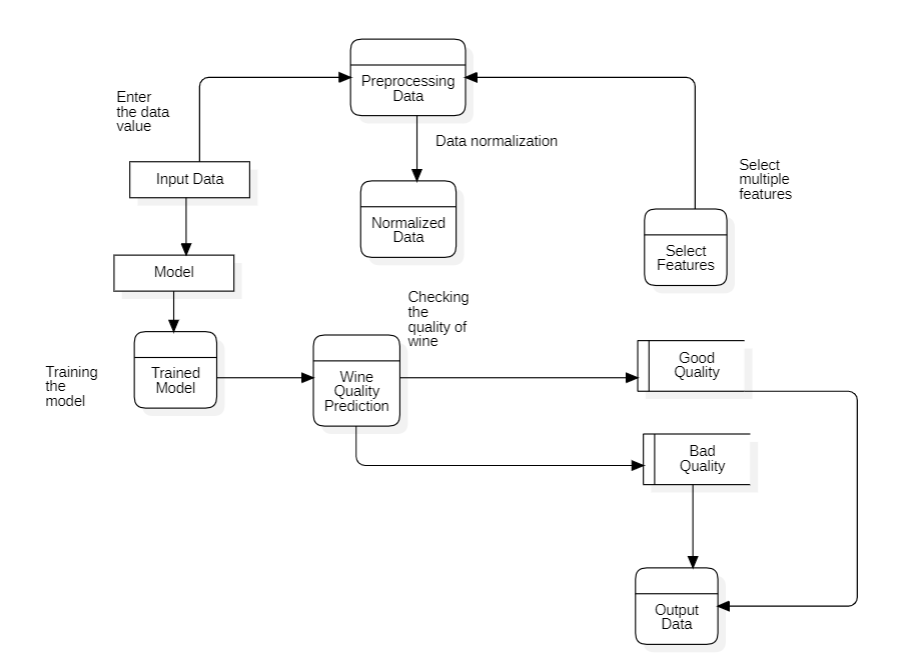
\includegraphics[width=0.9\linewidth]{./Wine DFD.png}
\caption{Data Flow Diagram}
\end{figure}
\pagebreak

\subsection{Timeline Chart }
\begin{figure}[h]
\centering
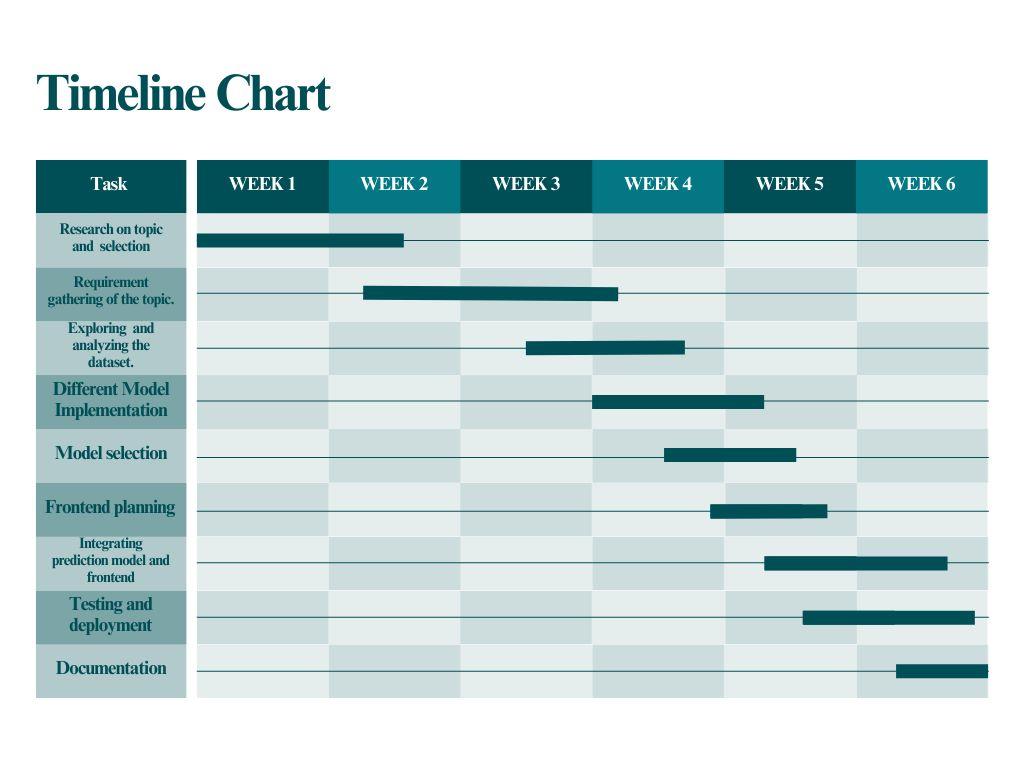
\includegraphics[width=1\linewidth]{Timeline chart.jpeg}
\caption{Timeline Chart}
\end{figure}
\pagebreak
\section{Algorithm }
\begin{figure}[h]
\centering
\includegraphics[width=0.8\linewidth]{algorithm.png}
\caption{Algorithm}
\end{figure}

\section{Feasibility Study }
\par A survey was undertaken to see whether the project was viable enough to operate in real time and was able to fulfil the needs of the markets. The primary goal of the study was to determine whether it could meet client needs and differentiate itself from other initiatives of a similar nature already on the market. The project underwent testing to determine its viability in the real world. The feasibility study may be conducted in a variety of ways and using a variety of approaches to examine every area.
There are 5 different type of feasibility study carried out. These are as follows:
1) Technical Feasibility
2) Economical Feasibility
3) Legal Feasibility
4) Operational Feasibility
5) Scheduling Feasibility

1) Technical Feasibility: The technical feasibility of a study on wine quality prediction is high as there are various machine learning algorithms and data mining techniques that can be used to predict wine quality based on different characteristics. Additionally, there is already a large amount of data available on wine production, making it possible to collect and pre-process data for machine learning models.

2) Economical Feasibility: The economical feasibility of a study on wine quality prediction can vary based on the cost of collecting and processing data, as well as the cost of using machine learning algorithms and data mining techniques. However, the potential benefits of the study, such as improved wine quality and increased customer satisfaction, may outweigh the costs in the long run.

3) Legal Feasibility: The legal feasibility of a study on wine quality prediction may involve complying with data privacy laws and regulations, as well as obtaining permission from vineyards and wineries to collect and use their data. However, as long as proper procedures are followed, a study on wine quality prediction can be legally feasible.

4) Operational Feasibility: The operational feasibility of a study on wine quality prediction may involve ensuring that the necessary infrastructure, equipment, and personnel are available to collect, process, and analyze data. Additionally, the study may require the use of specialized software and tools for machine learning and data mining.

5) Scheduling Feasibility: The scheduling feasibility of a study on wine quality prediction may depend on the availability of data and resources needed for the study. Additionally, the study may require significant time for data collection and pre-processing, as well as time for developing and testing machine learning models. Proper planning and scheduling can ensure that the study is completed within the desired timeframe.
\newline
\newline
In light of this, it may be said that the project is marketable and ready for usage by the general public. It has a user-friendly, interactive interface. All of the previously described fundamental features are present. It is compatible with the capabilities of providing the exact prediction about the inputed wine.
\pagebreak
\subsection{Wine Quality prediction Stats}
\begin{figure}[h]
\centering
\includegraphics[width=1\linewidth]{./digilock.png}
\caption{Digi Locker Stats}
\end{figure}

\chapter{Results and Discussion}
\section{Code}
\begin{lstlisting}
from flask import Flask, render_template, request
from sklearn.preprocessing import MinMaxScaler
import numpy as np
import pickle
import pandas as pd
import os

app = Flask(__name__)

model_path = 'model/model.sav'
csv_path = 'winequality-red.csv'

if not os.path.isfile(model_path):
    raise Exception(f"Model file not found at {model_path}")
if not os.path.isfile(csv_path):
    raise Exception(f"CSV file not found at {csv_path}")

Wine_model = pickle.load(open(model_path, 'rb'))


@app.route('/')
def index():
    return render_template('home.html')


@app.route('/predict', methods=['POST'])
def predict():
fixed_acidity = request.form.get('fixed_acidity', type=float)
volatile_acidity = request.form.get('volatile_acidity', type=float)
citric_acid = request.form.get('citric_acid', type=float)
residual_sugar = request.form.get('residual_sugar', type=float)
chlorides = request.form.get('chlorides', type=float)
free_sulfur_dioxide=request.form.get('free_sulfur_dioxide',type=float)
total_sulfur_dioxide=request.form.get('total_sulfur_dioxide',type=float)
density = request.form.get('density', type=float)
pH = request.form.get('pH', type=float)
sulphates = request.form.get('sulphates', type=float)
alcohol = request.form.get('alcohol', type=float)

# Check if any of the fields are empty
if None in [fixed_acidity, volatile_acidity, citric_acid, 
residual_sugar, chlorides,free_sulfur_dioxide, 
total_sulfur_dioxide, density, pH, sulphates, alcohol]:
return render_template('home.html', error_msg='Please 
fill in all the fields.')

    # Load the dataset and scale the input data
    dataset = pd.read_csv('winequality-red.csv')
    dataset_X = dataset.iloc[:, 
    [0, 1, 2, 3, 4, 5, 6, 7, 8, 9, 10]].values
    sc = MinMaxScaler(feature_range=(0, 1))
    dataset_scaled = sc.fit_transform(dataset_X)

    input_data = [[fixed_acidity, volatile_acidity, citric_acid, 
    residual_sugar, chlorides,free_sulfur_dioxide, 
    total_sulfur_dioxide, density, pH, sulphates, alcohol]]
    transformed_data = sc.transform(input_data)

    # Load the model and make a prediction
    Wine_model = pickle.load(open('model/model.sav', 'rb'))
    prediction = Wine_model.predict(transformed_data)

    # Check the prediction and show the appropriate template
    if prediction == 0:
        msg = 'Good quality wine'
        return render_template('goodwine.html', prediction=msg, 
        input_data=input_data[0])
    else:
        msg = 'Bad quality wine'
        return render_template('badwine.html', prediction=msg, 
        input_data=input_data[0])

if __name__ == '__main__':
    app.run(debug=True)

\end{lstlisting}
\pagebreak

\section{Software Results }
\par 
The software is a Flask web application that provides a user interface for predicting the quality of red wine based on 11 input features: fixed acidity, volatile acidity, citric acid, residual sugar, chlorides, free sulfur dioxide, total sulfur dioxide, density, pH, sulphates, and alcohol. These features are common factors that influence the taste and quality of wine.
The application works by first loading a pre-trained machine learning model, which has been trained on a dataset of red wine qualities. The model is capable of taking in the input features and predicting the quality of the wine.
When a user submits the wine feature values through a web form, the application scales the input data using MinMaxScaler, a popular data scaling method that scales the input data to be within a specified range, usually between 0 and 1. The scaled input data is then fed into the machine learning model to make a prediction.
The application then returns a message to the user indicating whether the predicted wine quality is good or bad. If the quality is good, it will show a page with a message saying so, and if the quality is bad, it will show a different page with a message indicating that the wine is of bad quality. The page also displays the input data along with the prediction, which helps the user understand how the wine quality was predicted.
The application is designed to be user-friendly and handles errors such as missing input fields gracefully. Overall, this software can be useful for wine enthusiasts, wine sellers, and anyone who wants to predict the quality of red wine based on certain input features.
\pagebreak

\section{Screen Shots }
\begin{figure}[h]
\centering
\\
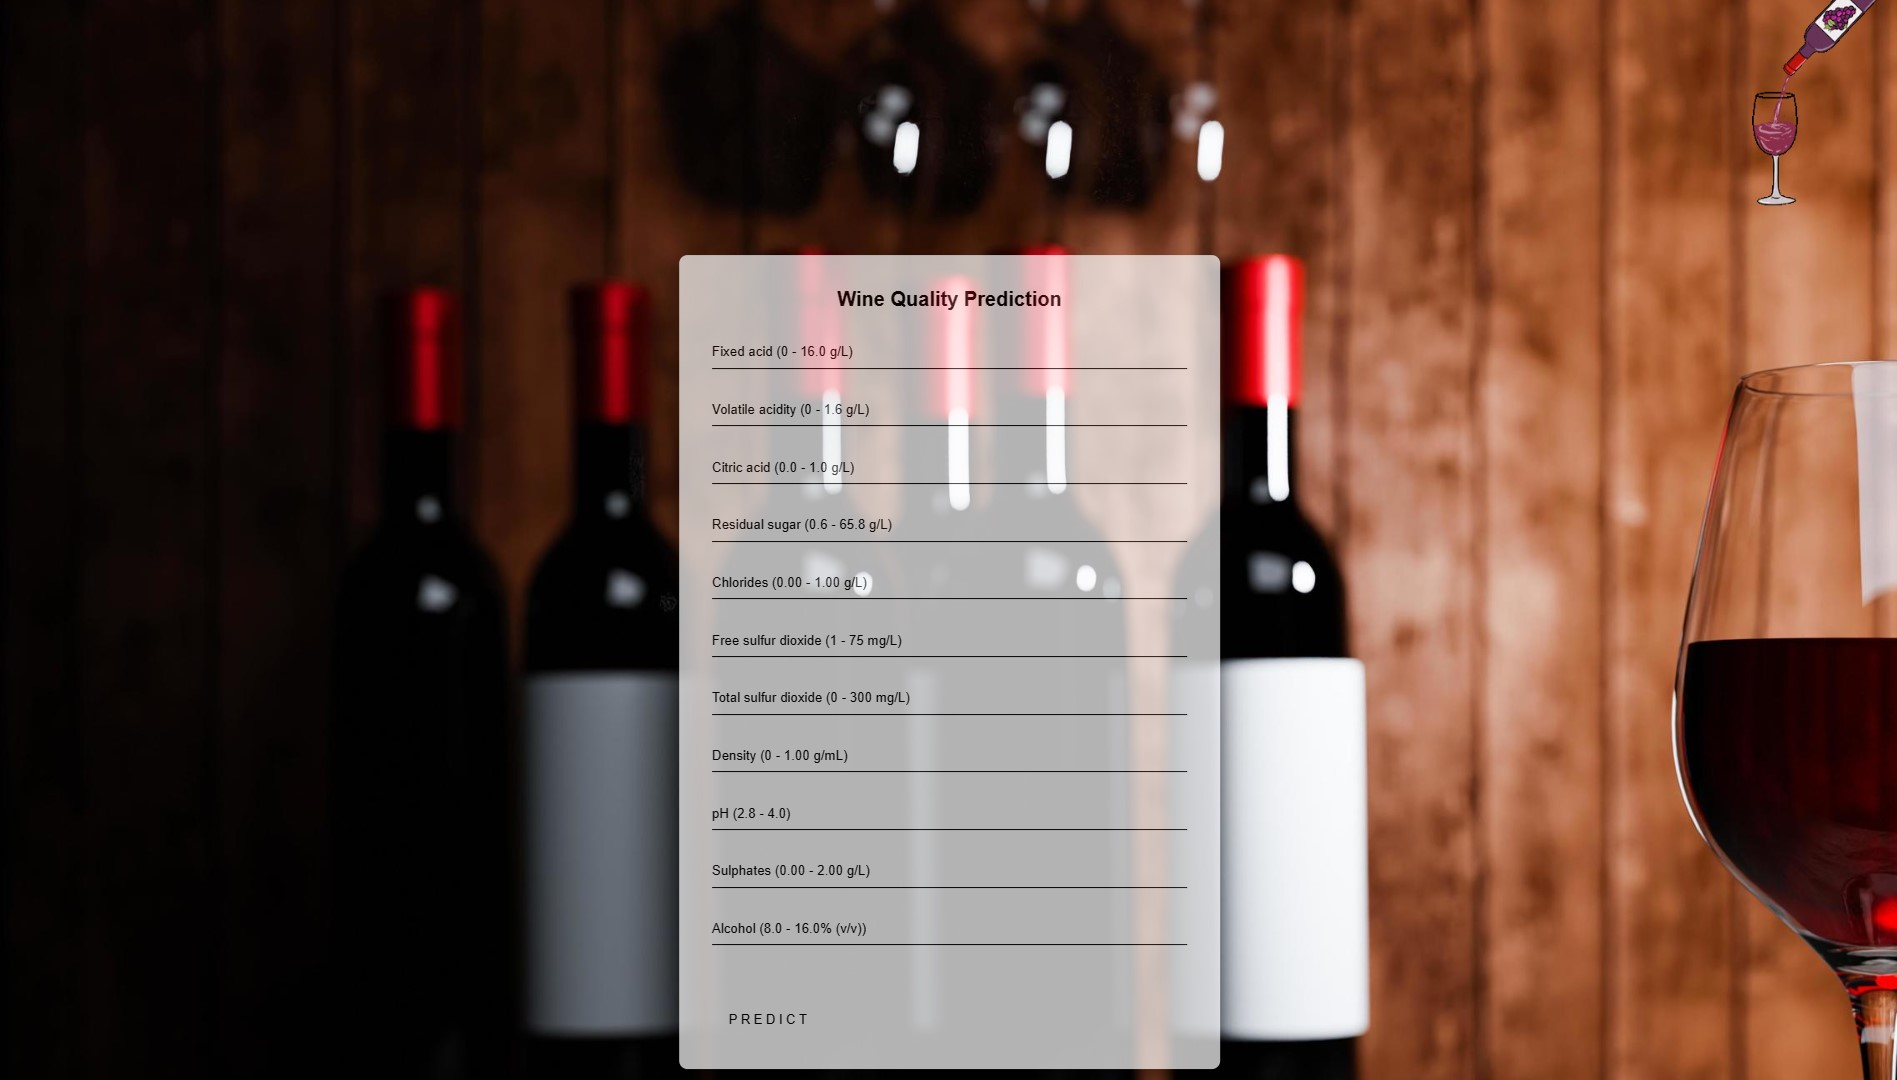
\includegraphics[width=1\linewidth, frame]{SS/H.jpg}
\linebreak
\caption{Home Page}
\linebreak
\\
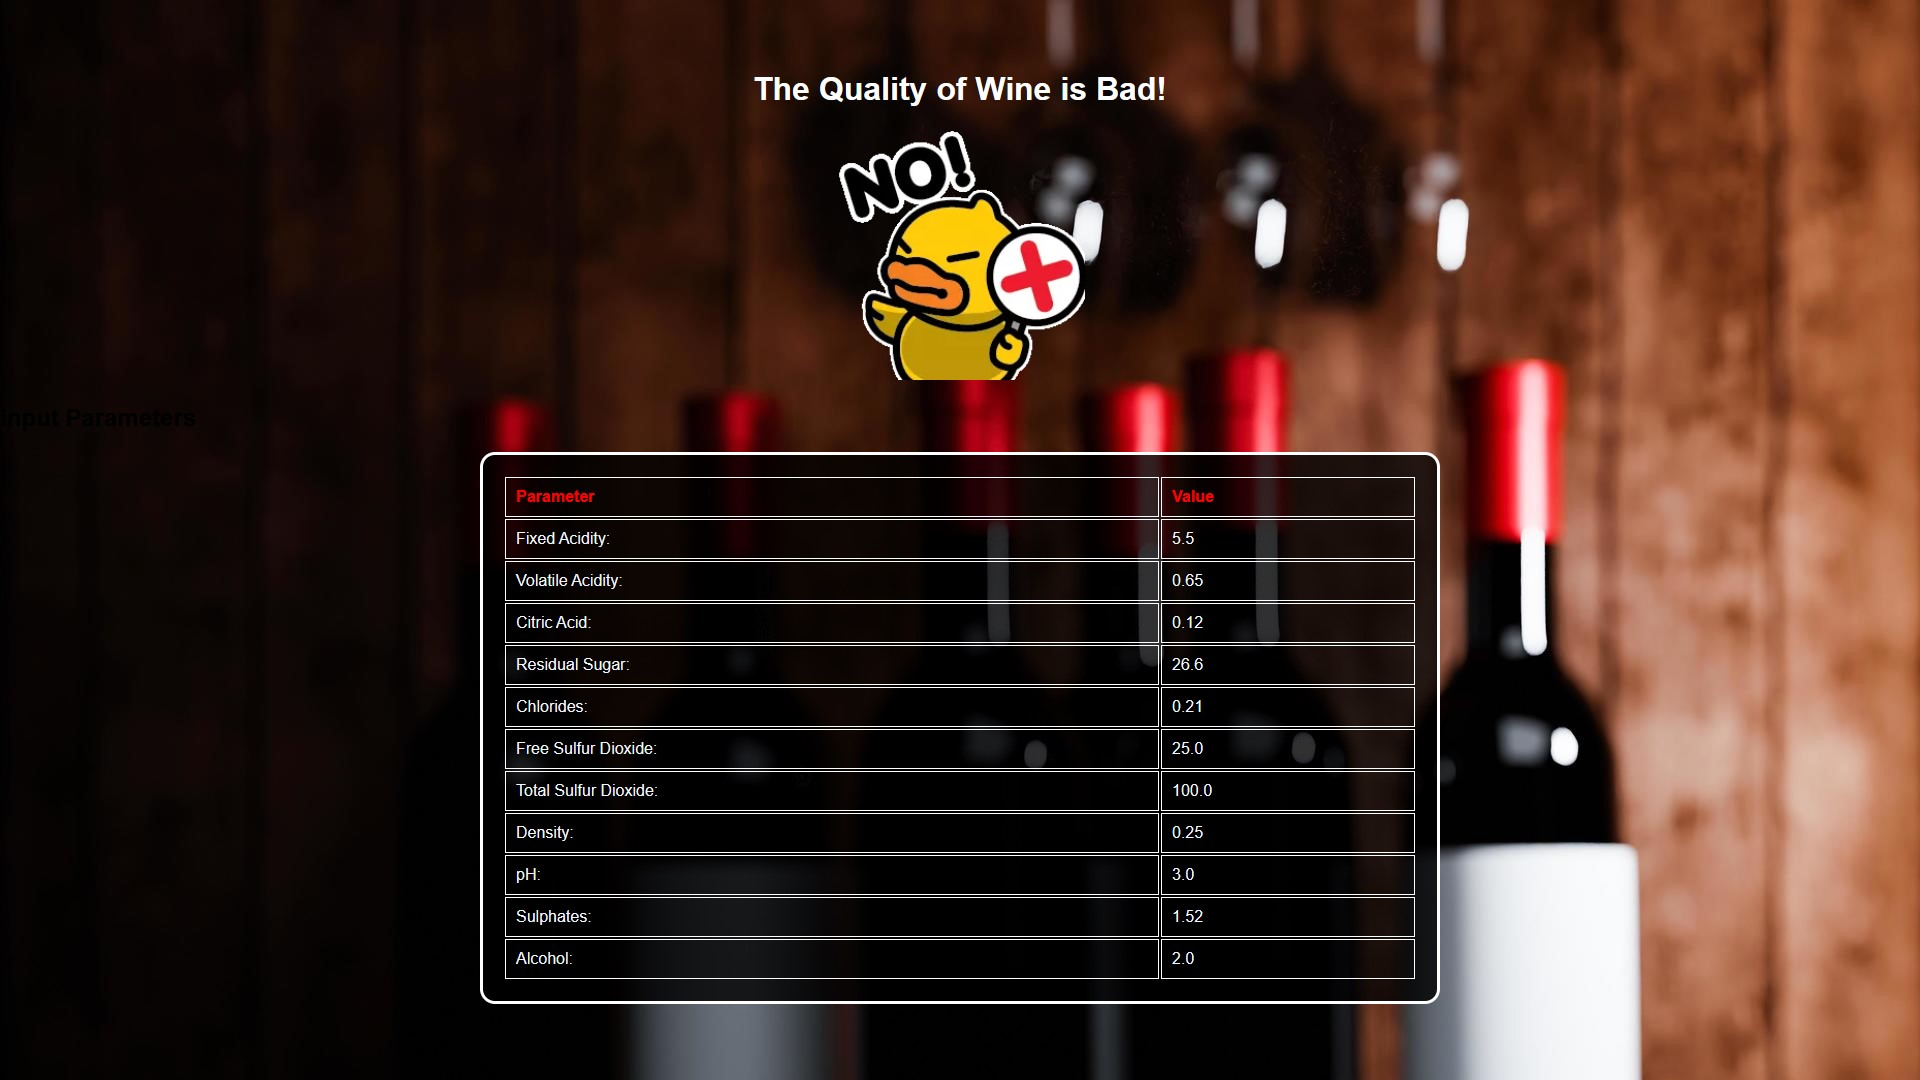
\includegraphics[width=1\linewidth, frame]{SS/B.jpg}
\linebreak
\caption{Good Wine}
\\
\end{figure}

\linebreak
\linebreak
\begin{figure}[h]
\centering
\\
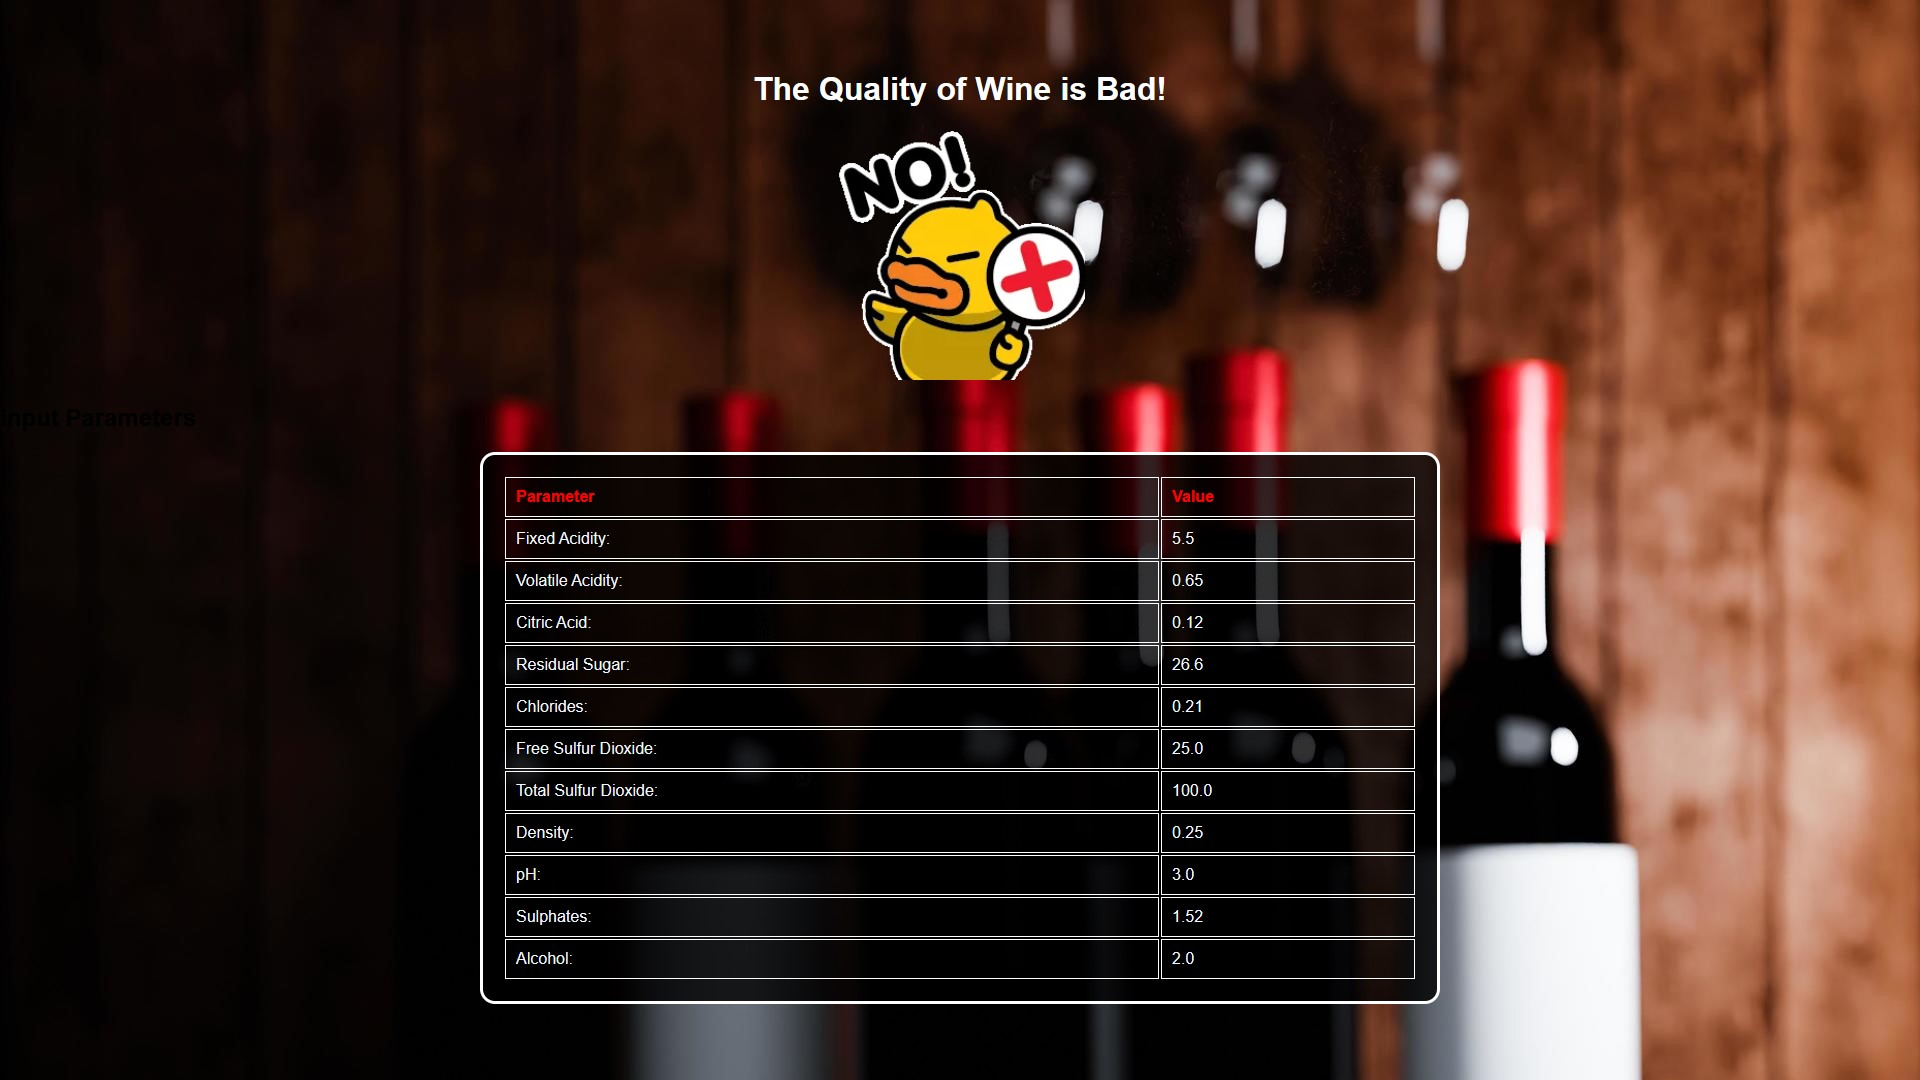
\includegraphics[width=1\linewidth,frame]{SS/B.jpg}
\linebreak
\caption{Bad Wine}
\\
\end{figure}

\pagebreak

\section{Testing Results }

\begingroup
\centering
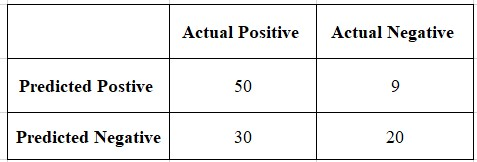
\includegraphics[width=0.8\linewidth]{SS/P.JPG}
\captionof{table}{Test Report - 1}
\vspace{12pt}
\endgroup

\par Precision = 50/(50 + 40) = 0.625
\par Accuracy = 80/109 = 0.733
\newline

\section{Test Case Report }
\linebreak
\par The test case report indicates the performance metrics for a prediction model. Precision is the proportion of true positives (correctly identified positive instances) among all the instances predicted as positive. In this case, the precision for prediction is 62.13, which means that out of all the positive predictions made by the model, 62.13 were actually true positives.

The accuracy of the prediction model is the proportion of correct predictions made by the model among all the predictions made. In this case, the accuracy for prediction is 73.33, which means that the model correctly predicted 73.33 of the instances.

It is important to note that these performance metrics can be influenced by factors such as the quality of the input data, the complexity of the model, and the selection of the evaluation metrics. Therefore, it is important to thoroughly evaluate the performance of a model using a variety of metrics and test cases to ensure that it performs well in different scenarios.

\pagebreak
\section{Additional details of the Project}
\par The machine learning model used in this software is a classification model, specifically a binary classifier. It is trained on a dataset of red wine samples with labels indicating whether the quality is good or bad.
The model is loaded using the Python library pickle, which allows for the serialization and deserialization of Python objects, including machine learning models. This makes it easy to load a pre-trained model into the application.
The input data is scaled using the MinMaxScaler method, which scales the data to a specified range, typically between 0 and 1. This is a common preprocessing step in machine learning, as it can improve the performance of the model.
The application is built using the Flask web framework, which is a popular Python framework for building web applications. Flask provides a simple and flexible way to create web applications, and it is well-suited for small to medium-sized projects.
The web form used to collect the input data is built using HTML and styled using CSS. Flask provides a simple templating system that makes it easy to incorporate HTML and CSS into the application.
The software is designed to be user-friendly, with error handling to ensure that the user enters all the required input data. If any input field is left empty, the application displays an error message asking the user to fill in all the fields.
The application is run using the Flask development server, which is not intended for production use. In a production environment, the application would typically be deployed using a production-grade web server such as Apache or Nginx.

\chapter{Conclusion}
\section{Summary}
\par According to our research, there is currently no website available on the market that can store all of the patient's medical records in one location. Additionally, if a website is able to accomplish this, they are not secure and run the highest risk of misplacing or altering crucial medical records. Because they provide no assurance of their security protocols, patients don't prefer this type of website because it could result in significant loss.We also noticed that our website is simple to use, access, and comprehend. Document updates and deletions are simple and only require the click of a single button.Our website guarantees the confidentiality, authenticity, and integrity of the medical reports patients publish on the internet because no patient's private information is disclosed. Additionally, the website offers simultaneous assistance to three different groups of people. Each user of the website is given the option to log in differently and is limited to using the features that are specific to their role on the website.
\section{Future Scope}
\par As a result, the website is fully equipped to aid in the expansion of the medical industry inside the online space. The website facilitates people's daily tasks and, like all digital platforms, improves people's quality of life.Additional functionality could be added to the website in the future, such as tools that allow patients to compare doctors based on patient reviews and then schedule an appointment. The website might also offer functions like the ability to acquire medications online by sending the pharmacy a prescription directly from the website.

\newpage
\bibliographystyle{plain}
\begin{thebibliography}{15}
\bibitem{1} 
Purushottam Arvind Petare (Sanjay Ghodawat Group of Institutions)
\\{GE-INTERNATIONAL JOURNAL OF MANAGEMENT   RESEARCH \\ VOLUME - 3, ISSUE- 6 (June 2015) IF-4.316 ISSN: (2321-1709)}
 \bibitem{2} 
Harpreet Kaur, Ushveen Kaur
\textit{International Journal of Recent Technology and \\Engineering (IJRTE)
ISSN: 2277-3878 (Online), Volume-8 Issue-4, November 2019}
\bibitem{3}
Pure Storage, https://www.purestorage.com/knowledge/what-is-ehr-storage.html
\textit{"EHR Storage"} 6th October 2022
\bibitem{4}
Razorpay, https://razorpay.com/docs/x/get-started/test-mode/
\textit{"RazorPay Test Mode"} 29th October 2022
\bibitem{5} 
International Research Journal of Engineering and Technology (IRJET)
\textit{Review on Medical Reports Extraction and Storage in EHR systems } 30th September 2022
\bibitem{6}
CodeWithHarry, https://www.youtube.com/watch?v=BLl32FvcdVM&ab
\textit{"Node.js Tutorial"} 1th October 2022
\bibitem{7}
CodeWithHarry, https://youtu.be/oSIv-E60NiU
\textit{"MongoDB Tutorial"} 1th October 2022
\bibitem{8}
Cuttly, https://cutt.ly/cNLGYXe
\textit{"DigiLocker Research Paper"} 6th October 2022
\end{thebibliography}

\end{document} 
